%
% a section on UML diagrams
% 
% \appendix
\section{Sample UML Diagrams}
\begin{description}
% A---------------------------------------------------------------
\item[Activity Diagram]  A UML diagram that demonstrates how users
interact with a given application, data flows, and branching options
for workflows and processes.
\begin{figure}[h!]
\center{\fbox{%
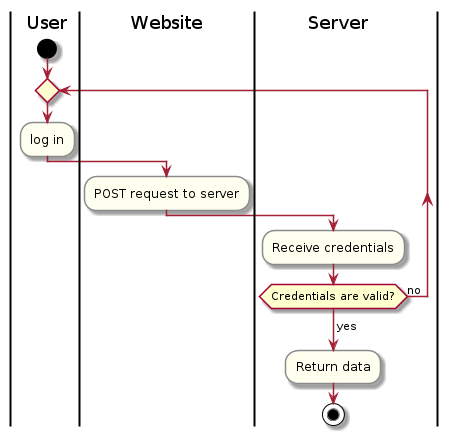
\includegraphics[width=0.70\textwidth]{activity-diagram-example}}}
\caption[Activity Diagram Example]{
This is a sample activity diagram, see text for explanation.}
\end{figure}

% C---------------------------------------------------------------
\item[Class Diagram] A UML diagram that demonstrates the various classes
in software, the relationships between those classes and how they depend
on each other.
\begin{figure}[h!]
\center{\fbox{%
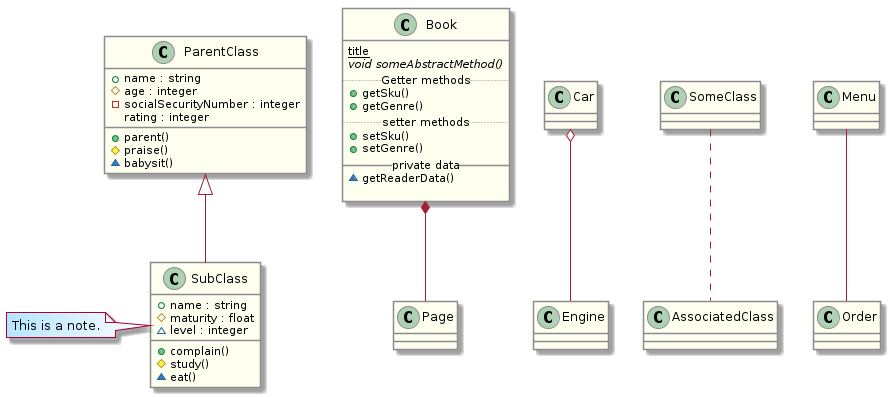
\includegraphics[width=0.70\textwidth]{class-diagram-example}}}
\caption[Class Diagram Example]{
This is a sample class diagram, see text for explanation.}
\end{figure}

\item[Component Diagram] A UML diagram that demonstrates how the modular
parts of software interact with each other using APIsi, interfaces
or other methods. The modular parts or components include databases,
web services, thin clients, thick clients, functions, libraries, and
other dependencies.
\begin{figure}[h!]
\center{\fbox{%
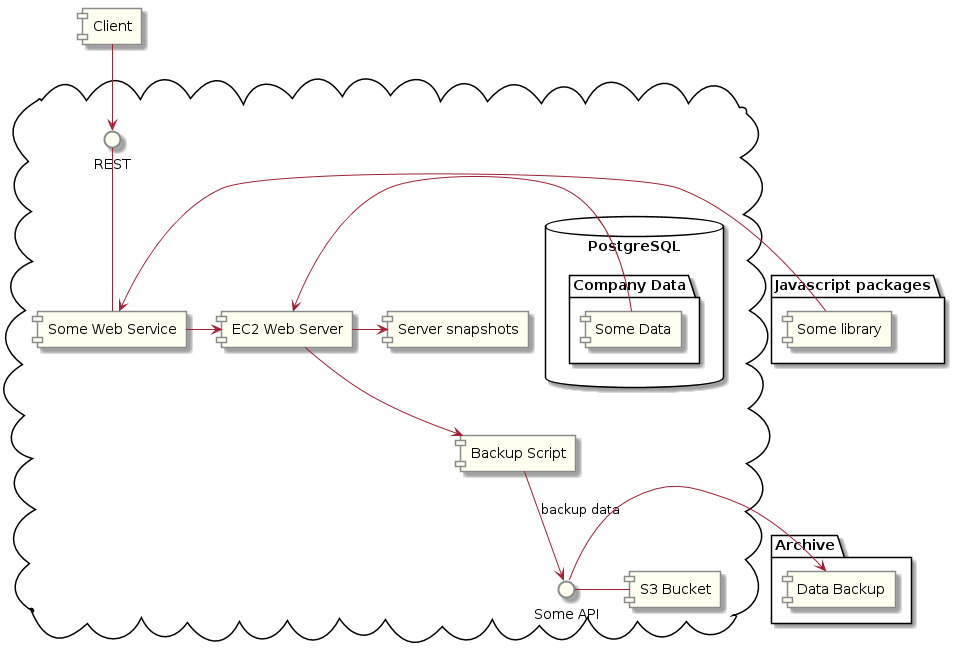
\includegraphics[width=0.70\textwidth]{component-diagram-example}}}
\caption[Component Diagram Example]{
This is a sample component diagram, see text for explanation.}
\end{figure}

% S---------------------------------------------------------------
\item[State Diagram] A UML diagram that describes the behavior and state
of the software.
\begin{figure}[h!]
\center{\fbox{%
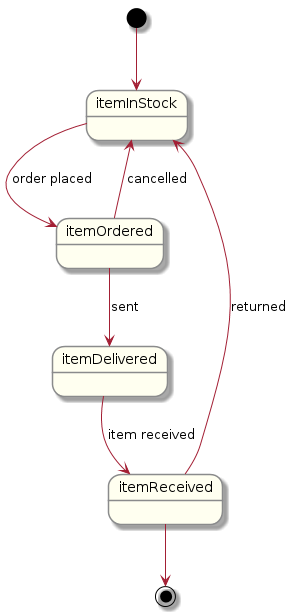
\includegraphics[width=0.70\textwidth]{state-diagram-example}}}
\caption[State Diagram Example]{
This is a sample state diagram, see text for explanation.}
\end{figure}

\end{description}

%
% eof
%
